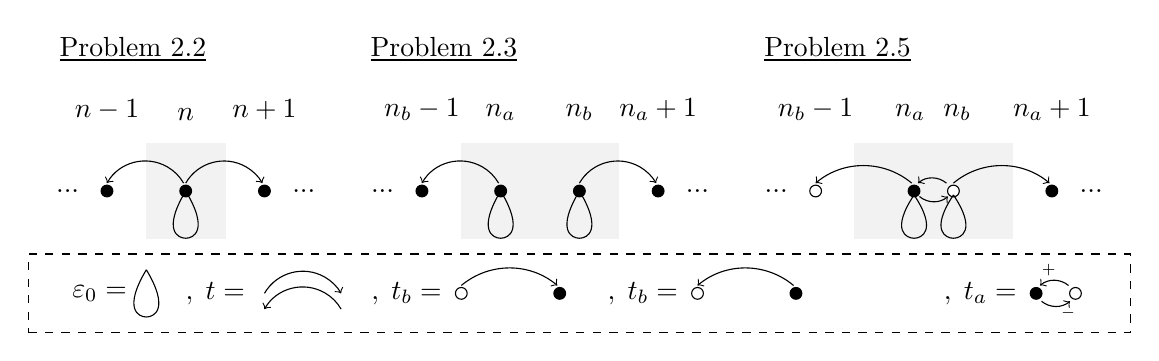
\begin{tikzpicture}[label distance = 0.7cm,
        mydot2/.style={circle, fill=white, draw, outer sep=0pt, inner sep=1.5pt},
        mydot1/.style={circle, fill=black, draw, outer sep=0pt, inner sep=1.5pt}]
        %%%%%%%%%% Label
            \node[label={[label distance = 0cm]east:{\underline{Problem 2.2}}}] at (-0.85,1.8) {};
            \node[label={[label distance = 0cm]east:{\underline{Problem 2.3}}}] at (3.1,1.8) {};
            \node[label={[label distance = 0cm]east:{\underline{Problem 2.5}}}] at (8.1,1.8) {};
        
        
        %%%%%%%%%% Legend
            \draw[dashed] (-1,-1.8) -| (13,-0.8) -| (-1,-1.8);
            
            % Epsilon
            \draw (0.5,-1) .. controls (0.2,-1.5) and (0.4,-1.6).. (0.5,-1.6)
                    (0.5,-1.6) .. controls (0.6,-1.6) and (0.8,-1.5) .. (0.5,-1);
            \node[label={[label distance = 0cm]west:{$\varepsilon_0 = $}}] at (0.5,-1.3) {};
        
            % T
            \draw [<-] (2,-1.5) arc (150:30:16pt); \draw [->] (2,-1.3) arc (150:30:16pt);
            \node[label={[label distance = 0cm]west:{$,\; t = $}}] at (2,-1.3) {};
            
            % Ta
            \draw [->] (4.5,-1.2) arc (130:50:27pt); \node[mydot2] at (4.5,-1.3) {}; \node[mydot1] at (5.75,-1.3) {};
            \node[label={[label distance = 0cm]west:{$,\; t_b = $}}] at (4.5,-1.3) {};
            
            % Tb
            \draw [<-] (7.5,-1.2) arc (130:50:27pt); \node[mydot2] at (7.5,-1.3) {}; \node[mydot1] at (8.75,-1.3) {};
            \node[label={[label distance = 0cm]west:{$,\; t_b = $}}] at (7.5,-1.3) {};
            
            % Ta - Tb
            \node[mydot1] at (11.8,-1.3) {}; \node[mydot2] at (12.3,-1.3) {};
            \draw [<-] (11.85,-1.2) arc (130:50:8pt); \draw [<-,rotate=180,shift={(-24.08,0.2)}] (11.85,1.2) arc (130:50:8pt);
            \node[label={[label distance = 0cm]west:{$,\; t_a = $}}] at (11.8,-1.3) {};
            \node[label={[label distance = 0cm]west:{\tiny{$+$}}}] at (12.3,-1) {};
            \node[label={[label distance = 0cm]west:{\tiny{$-$}}}] at (12.55,-1.55) {};
            
        
        %%%%%%%%%% problem 2.2
    	\node at (-0.5,0) {...}; \node at (2.5,0) {...};
    	\filldraw[fill=black!5!white, draw=black!5!white] (0.5,-0.6) rectangle (1.5,0.6);
    	\node[mydot1,label={above:{$\ket{n-1}$}}] (N11) at (0,0) {};
    	\node[mydot1,label={above:{$\ket{n}$}}] (N12) at (1,0) {};
    	\node[mydot1,label={above:{$\ket{n+1}$}}] (N13) at (2,0) {};
    	
        	%interaction
            \draw [<-] (0,0.1) arc (150:30:16pt); \draw [->] (1,0.1) arc (150:30:16pt);
            \draw (1,0) .. controls (0.7,-0.5) and (0.9,-0.6).. (1,-0.6)
                    (1,-0.6) .. controls (1.1,-0.6) and (1.3,-0.5) .. (1,0);
                
    	%%%%%%%%%% problem 2.3
    	\node at (3.5,0) {...}; \node at (7.5,0) {...};
    	\filldraw[fill=black!5!white, draw=black!5!white] (4.5,-0.6) rectangle (6.5,0.6);
    	\node[mydot1,label={above:{$\ket{n_b-1}$}}] (N21) at (4,0) {};
        \node[mydot1,label={above:{$\ket{n_a}$}}] (N22) at (5,0) {};
    	\node[mydot1,label={above:{$\ket{n_b}$}}] (N23) at (6,0) {};
    	\node[mydot1,label={above:{$\ket{n_a+1}$}}] (N24) at (7,0) {};

        	% interaction
        	\draw [<-] (4,0.1) arc (150:30:16pt); \draw [->] (6,0.1) arc (150:30:16pt);
            \draw (5,0) .. controls (4.7,-0.5) and (4.9,-0.6).. (5,-0.6)
                    (5,-0.6) .. controls (5.1,-0.6) and (5.3,-0.5) .. (5,0);
            \draw (6,0) .. controls (5.7,-0.5) and (5.9,-0.6).. (6,-0.6)
                    (6,-0.6) .. controls (6.1,-0.6) and (6.3,-0.5) .. (6,0);
                
    	%%%%%%%%%% problem 2.5
    	\node at (8.5,0) {...}; \node at (12.5,0) {...};
    	\filldraw[fill=black!5!white, draw=black!5!white] (9.5,-0.6) rectangle (11.5,0.6);
    	\node[mydot2,label={above:{$\ket{n_b-1}$}}] (N31) at (9,0) {};
    	\node[mydot1,label={above:{$\ket{n_a} \;$}}] (N32) at (10.25,0) {};
    	\node[mydot2,label={above:{$\; \ket{n_b}$}}] (N33) at (10.75,0) {};
    	\node[mydot1,label={above:{$\ket{n_a+1}$}}] (N34) at (12,0) {};

            % interaction
            \draw [<-] (9,0.1) arc (130:50:27pt); \draw [->] (10.75,0.1) arc (130:50:27pt);
            \draw [<-] (10.3,0.1) arc (130:50:8pt); \draw [<-,rotate=180,shift={(-20.98,-0.03)}] (10.3,0.1) arc (130:50:8pt);
            \draw (10.25,-0.05) .. controls (9.95,-0.5) and (10.15,-0.6).. (10.25,-0.6)
                    (10.25,-0.6) .. controls (10.35,-0.6) and (10.55,-0.5) .. (10.25,-0.05);
            \draw (10.75,-0.05) .. controls (10.45,-0.5) and (10.65,-0.6).. (10.75,-0.6)
                    (10.75,-0.6) .. controls (10.85,-0.6) and (11.05,-0.5) .. (10.75,-0.05);    
\end{tikzpicture}